% !TEX root = ../../I4PRJ, Grp3 - Dokumentation.tex
\section{Applikationslaget}
Dette afsnit beskriver implementeringen af applikationslaget. Implementeringen af applikationslaget består i, at implementere lagets modelklasser, presenterklasser og platform-specifikke user interface programmer. 

\subsection{Implementering af modelklasser}
Udvalgte dele af implementeringen af modelklasserne i applikationslaget beskrives i dette afsnit. Modelklasserne er implementeret i sproget C \#, i Microsoft Visual Studio. Den fulde implementering kan findes i Smartpool.Application.Model projektet.

\subsubsection{Session.cs}
Session-klassen indeholder hovedsageligt properties, som kan oversættes direkte fra klassens design til kode. Da Session klassen er designet som en Singleton, beskrives implementeringen af dens constructor og statiske Session medlem i dette afsnit.

Listing~\ref{code:application_model_ss} viser implementeringen af klassens statiske medlem. Når SharedSession bliver brugt første gang, laves en ny Session. I efterfølgende brug returneres den statiske session fra backing variablen sharedSession.

\begin{lstlisting}[caption={SharedSession},label={code:application_model_ss}]
public static Session SharedSession => _sharedSession ?? (_sharedSession = new Session());
\end{lstlisting}

Listing~\ref{code:application_model_sessionconstructor} viser implementeringen af Session-klassens constructor. Constructor'en er gjordt privat, således at SharedSession beskrevet i listing~\ref{code:application_model_ss}, er den eneste måde man kan oprette en Session.

\begin{lstlisting}[caption={Session constructor},label={code:application_model_sessionconstructor}]
private Session()
{
	SelectedPoolIndex = 0;
	Pools = new List<Tuple<string, bool>>();
}
\end{lstlisting}

\subsubsection{PoolLoader.cs}
PoolLoader-klassen indeholder en række metoder til at hente data fra connection-serveren. Generelt opretter metoder en passende besked fra Smartpool.Connection.Model, sender den med en IClientMessenger, og parser evt. svaret der modtages fra serveren.

Listing~\ref{code:application_model_gcdfp} viser implementeringen af en af disse metoder. I metoden oprettes en GetPoolDataRequestMsg som instantieres med sessionsinformation fra Session-klassen. Når svaret modtages, trækkes den relevante data ud af svarbeskeden, og laves om til en passende type.

\begin{lstlisting}[caption={GetCurrentDataFromPool(...)},label={code:application_model_gcdfp}]
public List<Tuple<SensorTypes, double>> GetCurrentDataFromPool(IClientMessenger clientMessenger)
{
	var request = new GetPoolDataRequestMsg(_session.UserName, _session.TokenString, false, _session.SelectedPool.Item1);
	var response = (GetPoolDataResponseMsg) clientMessenger.SendMessage(request);
	return response.SensorList.Select(sensor => new Tuple<SensorTypes, double>(sensor.Item1, sensor.Item2.LastOrDefault())).ToList();
}
\end{lstlisting}

Klassen indeholder også metoder der indlæser data i den statiske Session-instans. Metoden i listing~\ref{code:application_model_reloadpools} er et eksempel på dette. Metoden efterspørger pool-information fra serveren og gemmer den data der modtages i Session-instansen.

\begin{lstlisting}[caption={ReloadPools(...)},label={code:application_model_reloadpools}]
public void ReloadPools(IClientMessenger clientMessenger)
{
	var poolRequest = new GetPoolDataRequestMsg(_session.UserName, _session.TokenString, true);
	var response = (GetPoolDataResponseMsg) clientMessenger.SendMessage(poolRequest);
	_session.Pools = response.AllPoolNamesListTuple;
}
\end{lstlisting}

\subsubsection{PoolValidator.cs}
PoolValidator-klassen indeholder de properties der blev defineret i klassens design, samt implementeringen af de tilhørende funktioner. PoolValidator-klassens ansvar består i at tilbyde en måde, at validere pool-oplysninger. Metoden i listing~\ref{code:application_model_pvisvalid} definere hvornår en pool anses som værende godkendt i systemet. Som det fremgår af kodestykket, foretages en sammenligning af indholdet af klassens Name og SerialNumber properties.

\begin{lstlisting}[caption={IsValid()},label={code:application_model_pvisvalid}]
public bool IsValid()
{
	if (Name.Length == 0) return false;
	if (SerialNumber.Length == 0) return false;
	return true;
}
\end{lstlisting}

Klassen indeholder også funktionalitet, der tillader parsing af poolstørrelse og volumen, fra string til double-repræsentation. Listing~\ref{code:application_model_parsedvolume} implementerer denne funktionalitet. Metoden prøver først at parse klassens volume property hvis den indeholder en string, hvis ikke, prøver forsøger klassen at parse dimensions arrayet.

\begin{lstlisting}[caption={ParsedVolume()},label={code:application_model_parsedvolume}]
private double ParsedVolume()
{
if (_volume != "")
	{
	_dimensions[0] = ""; _dimensions[1] = ""; _dimensions[2] = "";
	try
	{
		var volume = double.Parse(_volume);
		return volume > 0 ? volume : 0;
	}
	catch (Exception)
		return 0;
}
else
 {
	 _volume = "";
	try
		return double.Parse(_dimensions[0]) * double.Parse(_dimensions[1]) * double.Parse(_dimensions[2]);
	catch (Exception)
		return 0;
	}
 }
\end{lstlisting}

\subsubsection{UserValidator.cs}
UserValidator-klassen indeholder de properties der blev defineret i klassens design, samt implementeringen af de tilhørende funktioner. Klassen kan validere brugeroplysninger, ved hjælp af de metoder der ses implementeret i listing~\ref{code:application_model_uservalidator}.

\begin{lstlisting}[caption={UserValidator valideringsmetoder},label={code:application_model_uservalidator}]
public bool PasswordIsValid => Passwords[0].Length >= MinimumCharacters && Passwords[0] == Passwords[1];
public bool IsValidForSignup => PasswordIsValid && Name.Length > 0 && Email.Length > 0;
public bool IsValidForLogin => Email.Length > 0 && Passwords[0].Length > 0;
\end{lstlisting}

Metoderne beskriver forskellige valideringsscenarier, og benytter klassens properties til at vurdere hvorvidt de indtastede oplysninger er tilstrækkelige.

\subsection{Implementering af presenter-klasser}
Udvalgte dele af implementeringen afpresenter-klasserne i applikationslaget beskrives i dette afsnit. Presenter-klasserne er udviklet i sproget C \#, i Microsoft Visual Studio. Den fulde implementering kan findes i Smartpool.Application.Presentation projektet. Presenter-klasserne implementerer de interfaces der er defineret i designet, samt metoder og parametre i de konkrete klassers design.

Fælles for alle presenter-klasserne er, at de implementerer en ViewDidLoad metode, da denne metode er defineret i IViewController interfacet. Et eksempel på en ViewDidLoad implementering ses i listing~\ref{code:application_impl_viewdidload}.

\begin{lstlisting}[caption={ViewDidLoad() i SignUpViewController.cs},label={code:application_impl_viewdidload}]
public void ViewDidLoad()
{
	_view.SetNameText("");
	_view.SetEmailText("");
	_view.SetPasswordText("");
	_view.SetPasswordValid(false);
	_view.SetButtonEnabled(false);
}
\end{lstlisting}

ViewDidLoad metoderne initiere view'ets state, ved at kalde view'ets interface-metoder. I eksemplet på listing~\ref{code:application_impl_viewdidload} ses det, at presenteren sætter tilstanden i view'ets tekstfelter og knapper. Dette er det generelle princip for alle ViewDidLoad metoderne, og derfor beskrives kun denne ene ViewDidLoad metode, indledningsvist.

Implementeringen af presenter-klassernes constructer-metoder er også ens i struktur. På listing~\ref{code:application_impl_presentercons} ses et eksempel på en af presenter-klassernes constructor. I constructor-metoden gemmes input parametrene i klassens private felter.

\begin{lstlisting}[caption={Constructor i SignUpViewController.cs},label={code:application_impl_presentercons}]
public SignUpViewController(ISignUpView view, IClientMessenger clientMessenger = null)
{
	_view = view;
	_clientMessenger = clientMessenger;
}
\end{lstlisting}

\subsubsection{SignUpViewController.cs}
Implementeringen af SignUpViewController-klassen bestod hovedsageligt i at sammenbinde ISignUpViewController-interfacets metoder, med handlinger der skulle foretages i SignUpViewController-klassens ISignUpView. Listing~\ref{code:application_impl_signupviewc1} viser et eksempel på en sådan sammenbinding, hvor en tekstændring modtages fra view'et, gemmes i en af klassens properties, og view'et opdateres.

\begin{lstlisting}[caption={DidChangeNameText(...)},label={code:application_impl_signupviewc1}]
public void DidChangeNameText(string text)
{
	User.Name = text;
	UpdateSignUpButton();
}
\end{lstlisting}

Klassens SignUp metode er implementeret således, at den kontakter connection-serveren, med de oplysninger som presenteren har kendskab til, om den bruger der ønskes oprettet. Metoden kan ses i listing~\ref{code:application_impl_signupmethod}. Når et svar modtages fra serveren, tjekker presenteren hvorvidt anmodningen var succesfuld. Herefter kaldes en metode i view'et, alt efter om anmodningen gik igennem eller ej. Hvis anmodningen blev afvist kaldes DisplayAlert i view'et.

\begin{lstlisting}[caption={SignUp()},label={code:application_impl_signupmethod}]
public void SignUp()
{
	var signUpRequest = new AddUserRequestMsg(User.Name, User.Email, User.Passwords[0]);
	var response = _clientMessenger.SendMessage(signUpRequest);
	var generalResponse = (GeneralResponseMsg) response;

	if (generalResponse.RequestExecutedSuccesfully)
		_view.SignUpAccepted();
	else
		_view.DisplayAlert("Invalid Sign Up", response.MessageInfo);
}
\end{lstlisting}

\subsubsection{LoginViewController.cs}
En del af LoginViewController-klassens metode implementering består i at sammenbinde kald fra view'et og tilhørende opdateringer af view'et, som i vist listing~\ref{code:application_impl_lvcdcet}.

\begin{lstlisting}[caption={DidChangeEmailText(...)},label={code:application_impl_lvcdcet}]
public void DidChangeEmailText(string text)
{
	User.Email = text;
	UpdateLoginButton();
}
\end{lstlisting}

Udover denne type metode, implementerer LoginViewController-klassen en Login metode, se listing~\ref{code:application_impl_lvclogin}, som igangsætter kommunikation med connection-serveren, og giver svaret tilbage til view'et. 

\begin{lstlisting}[caption={Login()},label={code:application_impl_lvclogin}]
 public void Login()
{
	var request = new LoginRequestMsg(User.Email, User.Passwords[0]);
	var response = _clientMessenger.SendMessage(request);
	var loginResponse = (LoginResponseMsg) response;

	if (loginResponse.LoginSuccessful)
	{
		// Save token
		var session = Session.SharedSession;
		session.TokenString = loginResponse.TokenString;
		session.UserName = User.Email;

		// Notify view
		_view.LoginAccepted (); 
	}
	else {
		// Reset password and display message
		_view.SetPasswordText("");
		_view.DisplayAlert("Login Error", loginResponse.MessageInfo);
	}
}
\end{lstlisting}

Login metoden konstruere en LoginRequestMsg, som den sender til serveren via. presenterens IClientMessenger. Når et svar modtages, tjekkes det hvorvidt anmodningen blev godkendt eller ej, og view'et opdateres.

\subsubsection{AddPoolViewController.cs}
AddPoolViewController-klassen skal i følge interfacet kunne håndtere tekstinput fra en række forskellige tekstfelter. Klassen implementerer derfor interface-metoden DidChangeText(...) med en switch-case, som set i listing~\ref{code:application_impl_apvcdct}. I kodestykket ses det, at presenter-klassen bruger en PoolValidator (kaldet pool), fra modellaget, til midlertidigt at gemme og validere den information der kommer ind, fra view'et.

\begin{lstlisting}[caption={DidChangeText(...)},label={code:application_impl_apvcdct}]
public void DidChangeText(AddPoolTextField textField, string text)
{
	// Switch based on text field type and set the proper variable
	switch (textField)
	{
	case AddPoolTextField.PoolName:
		Pool.Name = text;
		break;
	case AddPoolTextField.SerialNumber:
		Pool.SerialNumber = text;
		break;
	case AddPoolTextField.Volume:
		Pool.UpdateVolume(text, null);
		_dimensions[0] = ""; _dimensions[1] = ""; _dimensions[2] = "";
		break;
	case AddPoolTextField.Width:
		_dimensions[0] = text;
		Pool.UpdateVolume(null, _dimensions);
		break;
	case AddPoolTextField.Length:
		_dimensions[1] = text;
		Pool.UpdateVolume(null, _dimensions);
		break;
	case AddPoolTextField.Depth:
		_dimensions[2] = text;
		Pool.UpdateVolume(null, _dimensions);
		break;
	}

	// Update the pool button state since input could have changed the expected state
	UpdateAddPoolButton();
}
\end{lstlisting}

Interfacet indeholder også en metode der bliver kaldt af view'et, når en bruger ønskes oprettet. I listing~\ref{code:application_impl_apvcadbp} ses implementeringen af denne interface metode, i AddPoolViewController-klassen. I metoden oprettes en AddPoolRequestMessage og sendes til serveren. Godkendes svaret bruges en PoolLoader fra modellaget, til at indhente de opdaterede pool-oplysninger.

\begin{lstlisting}[caption={AddPoolButtonPressed()},label={code:application_impl_apvcadbp}]
public void AddPoolButtonPressed()
{
	if (!Pool.IsValid()) return;

	var userName = Session.SharedSession.UserName;
	var tokenString = Session.SharedSession.TokenString;

	// Send add pool request to server
	var addPoolMessage = new AddPoolRequestMsg(userName, tokenString, Pool.Name, Pool.Volume, Pool.SerialNumber);
	var response = _clientMessenger.SendMessage(addPoolMessage);
	var addPoolResponse = (GeneralResponseMsg) response;

	// Act on response
	if (addPoolResponse.RequestExecutedSuccesfully)
	{
		var loader = new PoolLoader();
		loader.ReloadPools(_clientMessenger);
		_view.PoolAdded();
	} else if (addPoolResponse.TokenStillActive == false)
		_view.DisplayAlert("Invalid action", response.MessageInfo);
}
\end{lstlisting}

\subsubsection{EditUserViewController.cs}
EditUserViewController-klassen skal i følge interfacet håndtere ændring af brugerens password. Klassen implementerer metoder der tager imod tekstinput view'et, same validerer de nye oplysninger med en UserValidator fra modellaget. I listing~\ref{code:application_impl_euvcdcnpw} ses implementeringen af den metode, der tager imod oplysninger om det nye password. Oplysningerne gemmes i password-array'et i UserValidator-objektet User. Herefter kaldes private hjælpemetoder, der opdatere view'ets tilstand, for at give feedback på, om de indtastede oplysninger kan godkendes eller ej.

\begin{lstlisting}[caption={DidChangeNewPasswordText(...)},label={code:application_impl_euvcdcnpw}]
public void DidChangeNewPasswordText(string text, int fieldNumber)
{
	if (fieldNumber > 1) throw new ArgumentException();
	User.Passwords[fieldNumber] = text;
	UpdatePassword();
	UpdateSaveButton();
}
\end{lstlisting}

Klassen implementerer også en SaveButtonPressed metode, som kaldes nå brugeren er tilfreds med de ændringer, vedkommende har foretaget. SaveButtonPressed metoden kalder hjælpemetoden Save, som ses i listing~\ref{code:application_impl_euvcsave}. Save metoden laver en ChangePasswordRequestMsg fra connection-model laget, og sender den til serveren. Svaret undersøges og view'et opdateres.

\begin{lstlisting}[caption={Save()},label={code:application_impl_euvcsave}]
public void Save()
{
	// Send message to client
	var updatePasswordRequest = new ChangePasswordRequestMsg(_session.UserName, _session.TokenString, _oldPassword, User.Passwords.First());
	var response = (GeneralResponseMsg) _clientMessenger.SendMessage(updatePasswordRequest);

	if (response.RequestExecutedSuccesfully)
		_view.UpdateSuccessful();
	else
		_view.DisplayAlert("Save Error", response.MessageInfo);
}
\end{lstlisting}

\subsubsection{EditPoolViewController.cs}
EditPoolViewController-klassen skal i følge interfacet håndtere ændring af de pools, der er tilknyttet en brugers konto. Klassen implementerer en DidChangeText-metode fra interfacet, på samme måde som AddPoolViewController (se listing~\ref{code:application_impl_apvcdct}, side~\pageref{code:application_impl_apvcdct}).

Klassen implementerer også metoder til at gemme eller slette pool-oplysninger. I listing~\ref{code:application_impl_epvcsd} ses implementeringen af SaveButtonPressed-metoden. I denne metode oprettes en UpdatePoolRequestMsg fra connection-model laget, som sendes til serveren. Svaret undersøges og view'et opdateres.

\begin{lstlisting}[caption={SaveButtonPressed()},label={code:application_impl_epvcsd}]
public void SaveButtonPressed()
{
	if (!_pool.IsValid()) return;

	var session = Session.SharedSession;
	var updatePoolMessage = new UpdatePoolRequestMsg(session.UserName, session.TokenString, session.SelectedPool.Item1, _pool.Name, _pool.Volume);
	var response = (GeneralResponseMsg) _clientMessenger.SendMessage(updatePoolMessage);

	// Act on the response from the server
	if (response.RequestExecutedSuccesfully)
	{
		_loader.ReloadPools(_clientMessenger);
		_view.PoolUpdated();
		LoadPoolInfoIntoView();
	}
	else
		_view.DisplayAlert("Save Error", response.MessageInfo);
}
\end{lstlisting}

EditPoolViewController indeholder også en privat hjælpemetode, der kalder IPoolDisplaying interface-metoderne i view'et, når view'et ønskes opdateret med pool-information. I listing~\ref{code:application_impl_pcdlpiiv} ses implementeringen af LoadPoolInfoIntoView-metoden, som bruger klassens PoolLoader fra modellaget, til at indlæse pool-oplysninger og derefter opdatere view'et.

\begin{lstlisting}[caption={LoadPoolInfoIntoView()},label={code:application_impl_pcdlpiiv}]
private void LoadPoolInfoIntoView()
{
	// Load active pool info into text fields
	_view.SetAvailablePools(_session.Pools);

	var volumeAndSerialNumber = _loader.GetVolumeAndSerialNumberForSelectedPool(_clientMessenger);

	if (_loader.PoolsAreAvailable())
	{
		// Update pool loader
		_pool.Name = _session.SelectedPool.Item1;
		_pool.UpdateVolume(string.Format($"{volumeAndSerialNumber.Item1}"), null);
		_pool.SerialNumber = volumeAndSerialNumber.Item2;

		// Update view
		_view.SetNameText(_session.SelectedPool.Item1);
		_view.SetSerialNumberText(_pool.SerialNumber);
		_view.SetVolumeText(string.Format($"{_pool.Volume}"));
		_view.SetSelectedPoolIndex(_session.SelectedPoolIndex);
		_view.SetSaveButtonEnabled(true);
		_view.SetDeleteButtonEnabled(true);
	}
	else
	{
		_view.DisplayAlert("No pools", "You have no pools to edit");
		_view.SetSaveButtonEnabled(false);
		_view.SetDeleteButtonEnabled(false);
	}
}
\end{lstlisting}

\paragraph{IPoolControlling}
EditPoolViewController, StatViewController og HistoryViewController implementerer alle IPoolControlling. De tre presenter-klasser implementerer IPoolControlling interfacet på samme måde. Implementeringen af IPoolControlling eksemplificeres derfor udelukkende i dette afsnit, ved visning af EditPoolViewController-klassens implementering af interface-metoden DidSelectPool, i listing~\ref{code:application_impl_pcdsp}.

\begin{lstlisting}[caption={DidSelectPool(...)},label={code:application_impl_pcdsp}]
public void DidSelectPool(int index)
{
	// Parse the name in the pool loader 
	_session.SelectedPoolIndex = index;
	if (!_loader.PoolsAreAvailable()) return;

	_view.SetNameText(_session.SelectedPool.Item1);
	_view.SetDeleteButtonEnabled(true);
}
\end{lstlisting}

\subsubsection{StatViewController.cs}
StatViewController-klassen håndterer indlæsning af pool-data til det tilknyttede view. I StatViewController-klassens ViewDidLoad, set i listing~\ref{code:application_impl_vdlstat}, bruges klassens PoolLoader til at indlæse pool-oplysninger i view'et.

\begin{lstlisting}[caption={ViewDidLoad() in StatViewController},label={code:application_impl_vdlstat}]
public void ViewDidLoad()
{
	// Load pools from server
	_loader.ReloadPools(_clientMessenger);

	// Load active pool info into text fields
	if (!_loader.PoolsAreAvailable())
		_view.DisplayAlert("No pools available", "You have not added any pools yet. Please go to 'Add Pool' to add a pool.");
	else
	{
		_view.SetAvailablePools(_session.Pools);
		_view.SetSelectedPoolIndex(_session.SelectedPoolIndex);
		LoadSensorData();
	}
}
\end{lstlisting}

ViewDidLoad-metoden benytter sig af en private hjælpemetode, LoadSensorData. Metoden, som ses i listing~\ref{code:application_impl_statlsd}, kalder view interface-metoden DisplaySensorData og bruger klassens PoolLoader, til at indlæse måleværdier i view'et.

\begin{lstlisting}[caption={LoadSensorData() in StatViewController},label={code:application_impl_statlsd}]
private void LoadSensorData()
{
	// Loads current sensor data into the view
	_view.DisplaySensorData(_loader.GetCurrentDataFromPool(_clientMessenger));
}
\end{lstlisting}

\subsubsection{HistoryViewController.cs}
HistoryViewController-klassen håndterer indlæsning af pool-data i det tilknyttede view. I HistoryViewController-klassen minder i implementering om StatViewController. ViewDidLoad, set i listing~\ref{code:application_impl_vdlhistory}, bruges klassens PoolLoader til at indlæse pool-oplysninger i view'et.

\begin{lstlisting}[caption={ViewDidLoad() in HistoryViewController},label={code:application_impl_vdlhistory}]
public void ViewDidLoad()
{
	// Load pools from server
	_loader.ReloadPools(_clientMessenger);

	// Load active pool info into text fields
	if (!_loader.PoolsAreAvailable())
		_view.DisplayAlert("No pools available", "You have not added any pools yet. Please go to 'Add Pool' to add a pool.");
	else
	{
		_view.SetAvailablePools(_session.Pools);
		_view.SetSelectedPoolIndex(_session.SelectedPoolIndex);
		LoadSensorData();
	}
}
\end{lstlisting}

ViewDidLoad-metoden benytter sig på samme måde som StatViewController, af en private hjælpemetode. Metoden, som ses i listing~\ref{code:application_impl_historylsd}, kalder view interface-metoden DisplayHistoricData og bruger klassens PoolLoader, til at indlæse historiske måleværdier i view'et.

\begin{lstlisting}[caption={LoadSensorData() in HistoryViewController},label={code:application_impl_historylsd}]
private void LoadSensorData()
{
	// Loads historic sensor data into the view
	_view.DisplayHistoricData(_loader.GetHistoricDataFromPool(_clientMessenger, 7));
}
\end{lstlisting}

\subsection{Implementering af view-klasser}
Applikationslagets view-interfaces er blevet implementeret af klasser på forskellige platforme, og beskrives derfor i deres egne afsnit. På figur~\ref{fig:view_family} illustreres de færdigimplementerede brugergrænseflader. 

\begin{figure}
	\centering
	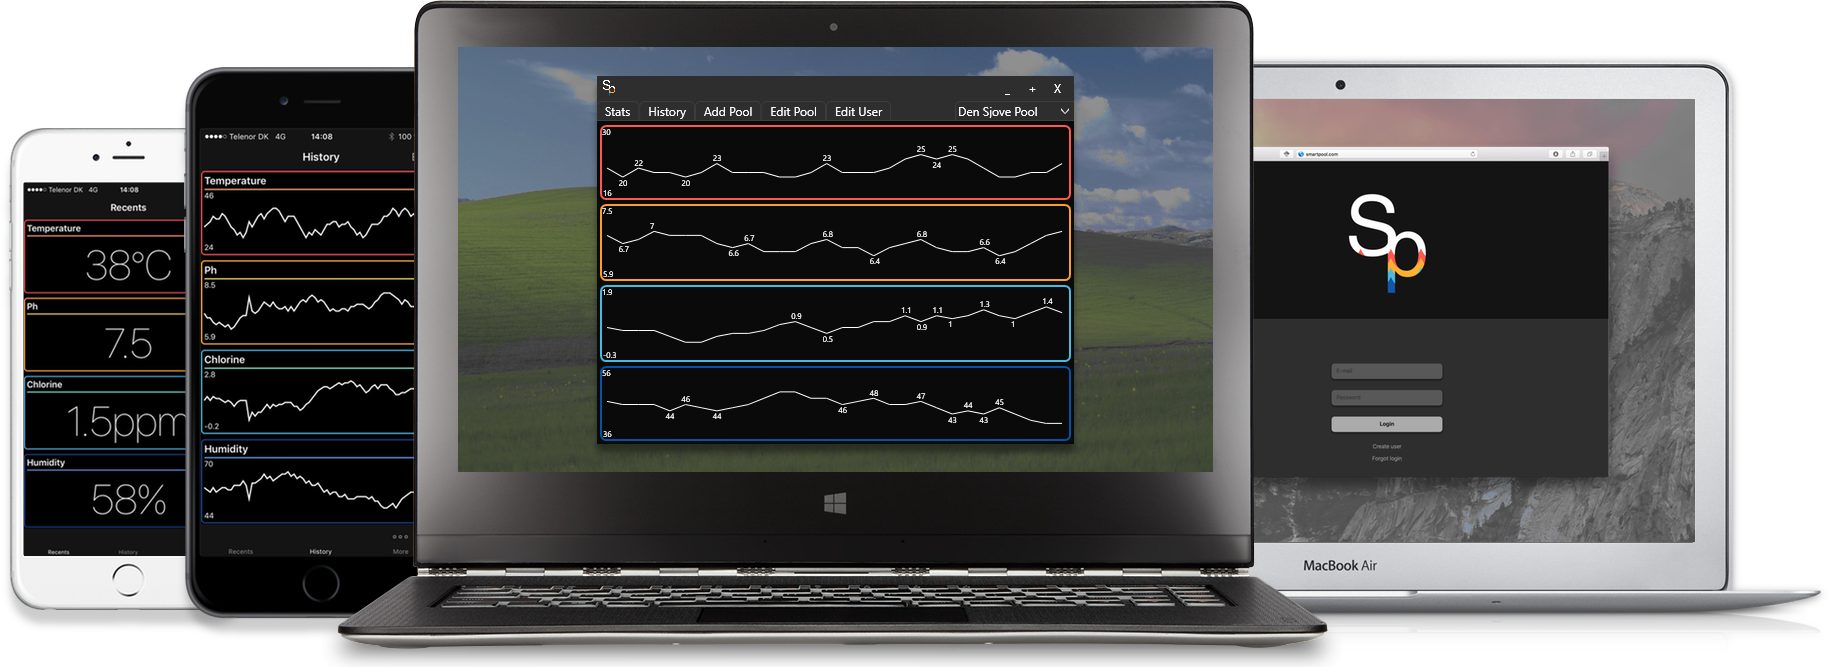
\includegraphics[width=1.0\linewidth]{figs/implementering/view_family}
	\caption{Brugergrænsefladeimplementering på hhv. iOS, Windows og Web}
	\label{fig:view_family}
\end{figure}